\listoffigures
\addcontentsline{toc}{chapter}{図目次}

\begin{figure}
    \centering
    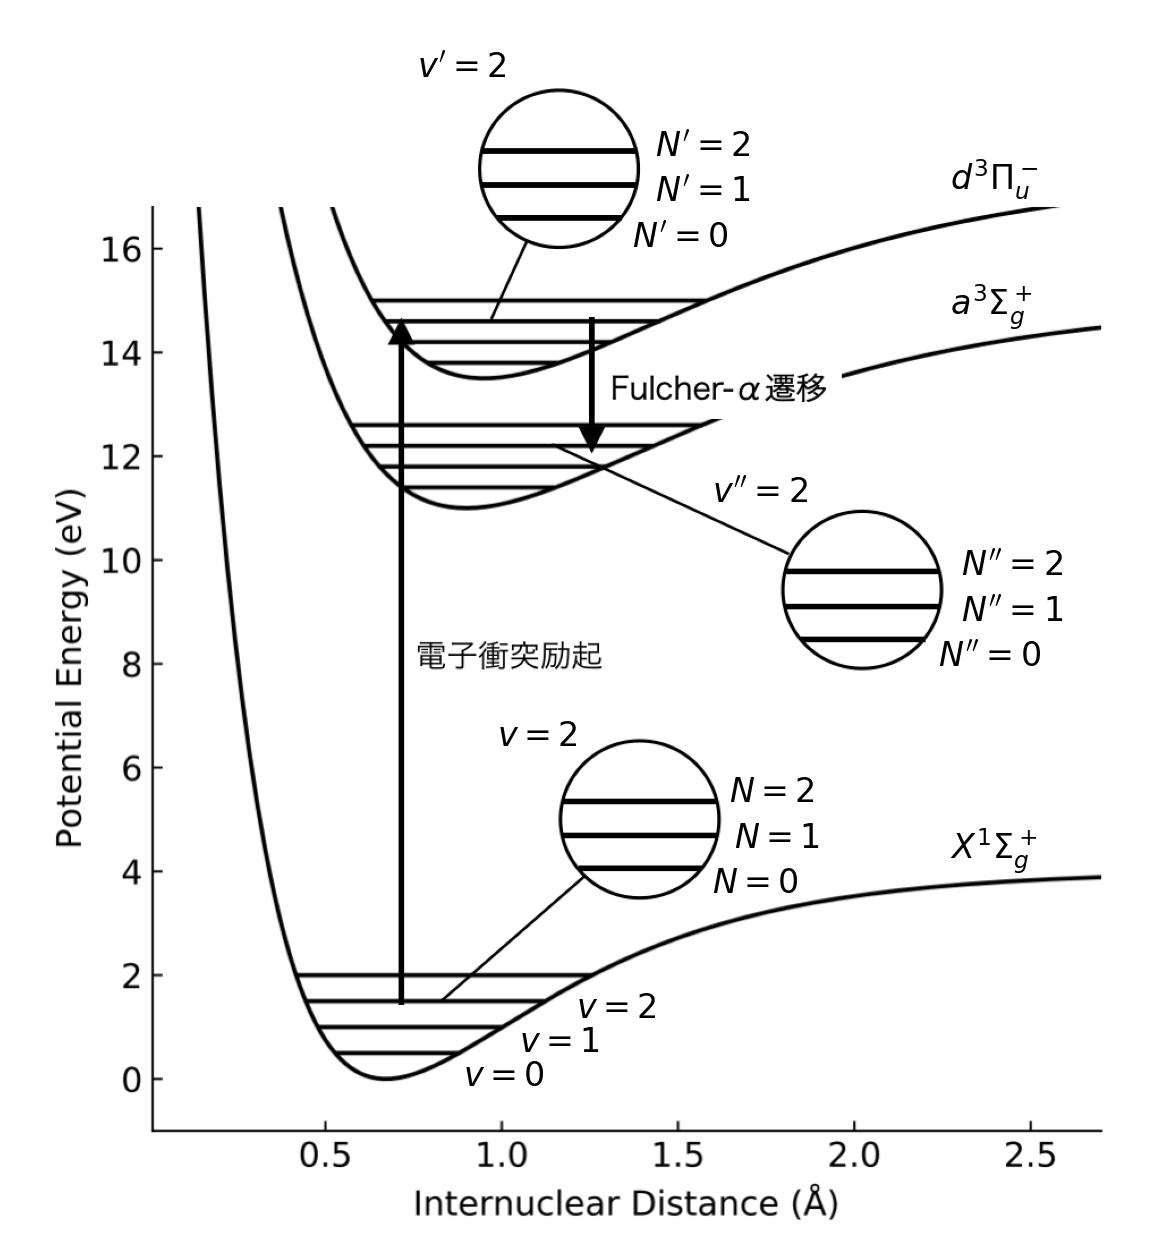
\includegraphics[width=15cm]{pictures/energy-level.png}
    \caption[$\rm{H}_2$のポテンシャル曲線]{$\rm{H}_2$のポテンシャル曲線.図中の$X^1 \Sigma^+_g$, $d^3 \Pi^-_u$, $a^3 \Sigma^+_g$はそれぞれ基底準位,発光上準位,発光下準位の電子準位であり,$v, v', v''$と$J, J', J''$はそれぞれ基底準位,発光上準位,発光下準位の振動量子数と回転量子数を表す.}
    \label{fig:energy-level}
\end{figure}

\begin{figure}
    \centering
    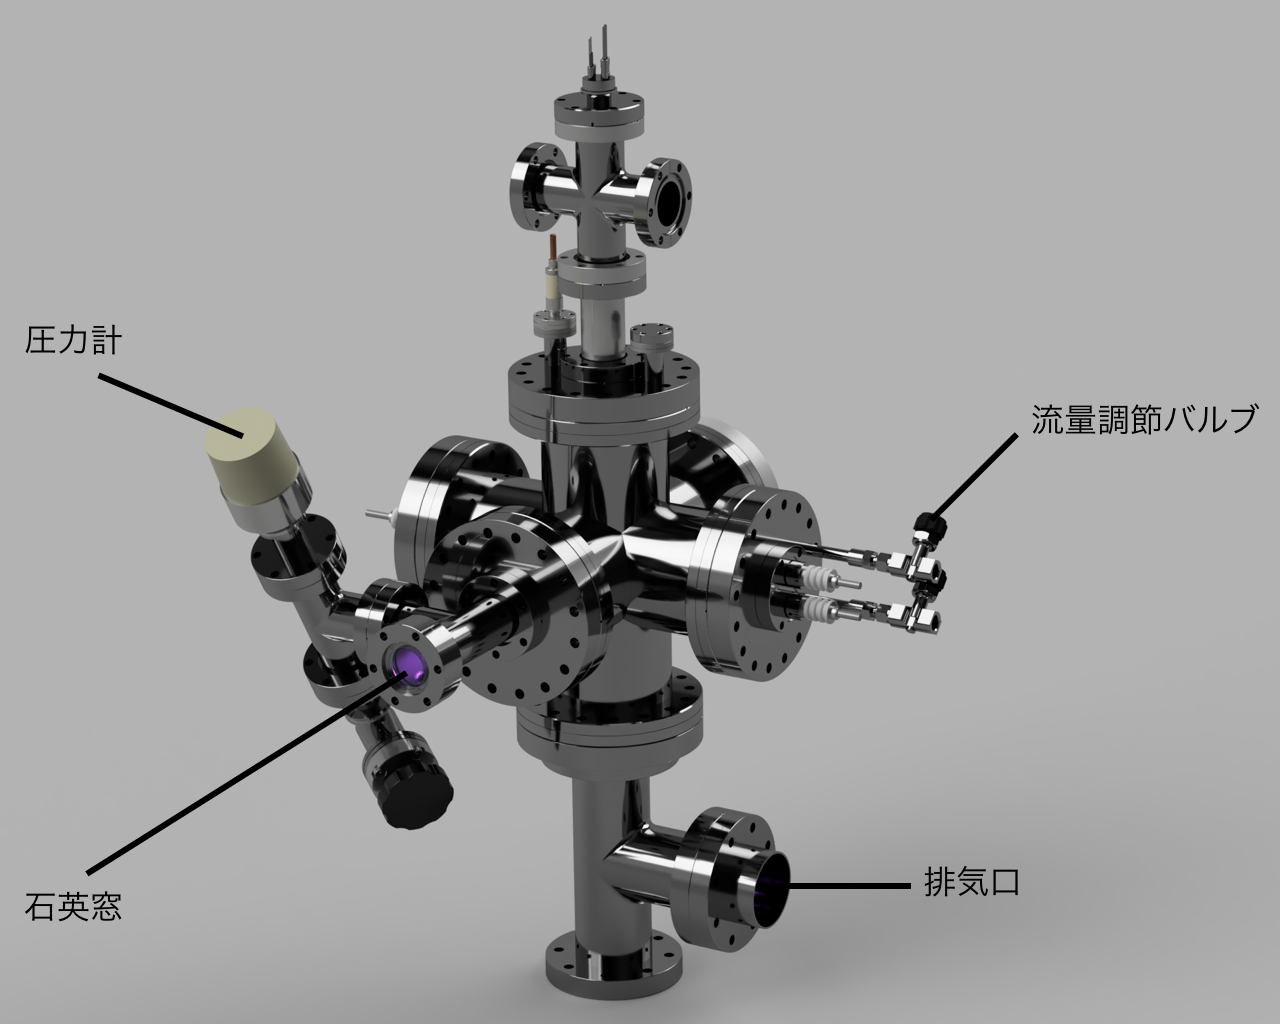
\includegraphics[width=15cm]{pictures/chamber-picture.png}
    \caption{プラズマチャンバの外観}
    \label{fig:chamber-picture}
\end{figure}

\begin{figure}
    \centering
    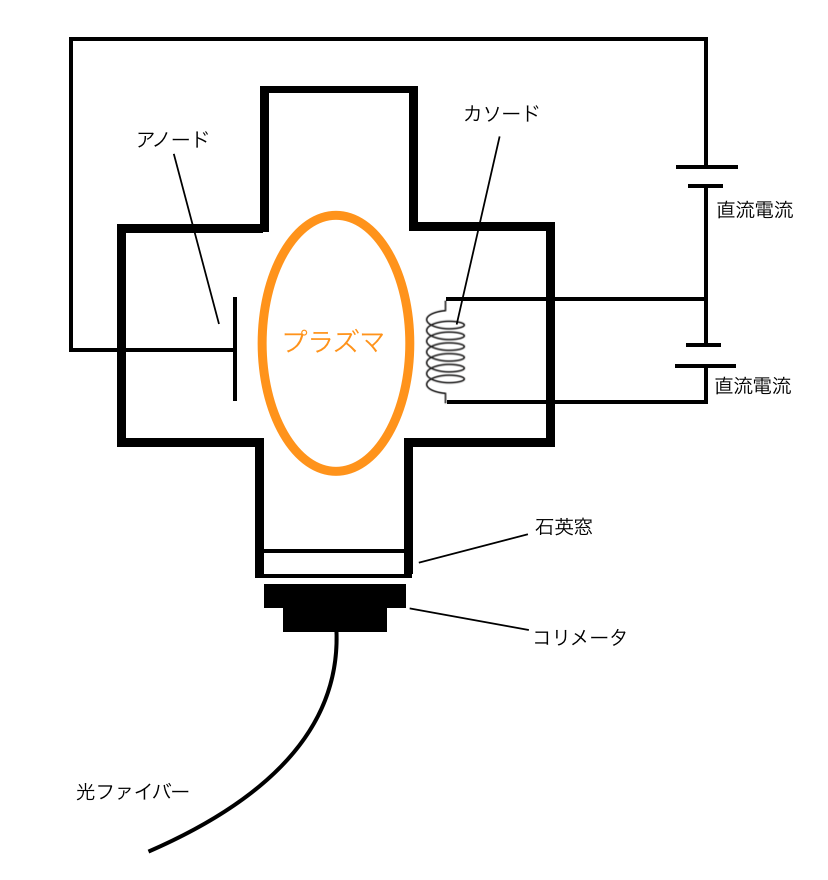
\includegraphics[width=15cm]{pictures/chamber-simple.png}
    \caption{プラズマチャンバの構造の簡略図}
    \label{fig:chamber-simple}
\end{figure}

\begin{figure}
    \centering
    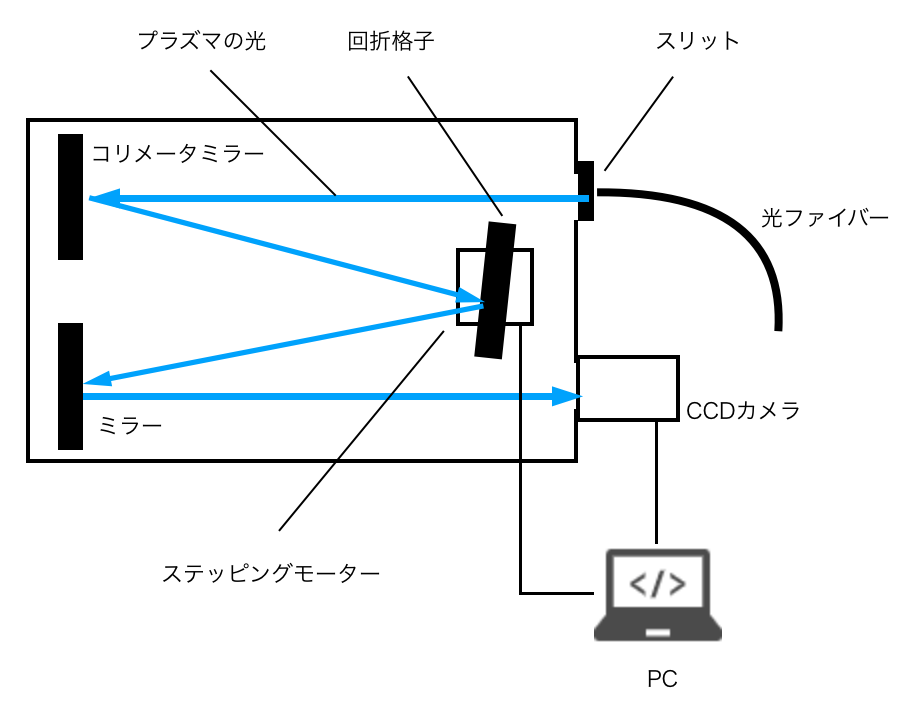
\includegraphics[width=15cm]{pictures/spectrometer-picture.png}
    \caption{分光器の簡略図}
    \label{fig:spectrometer-picture}
\end{figure}

\begin{figure}
    \centering
    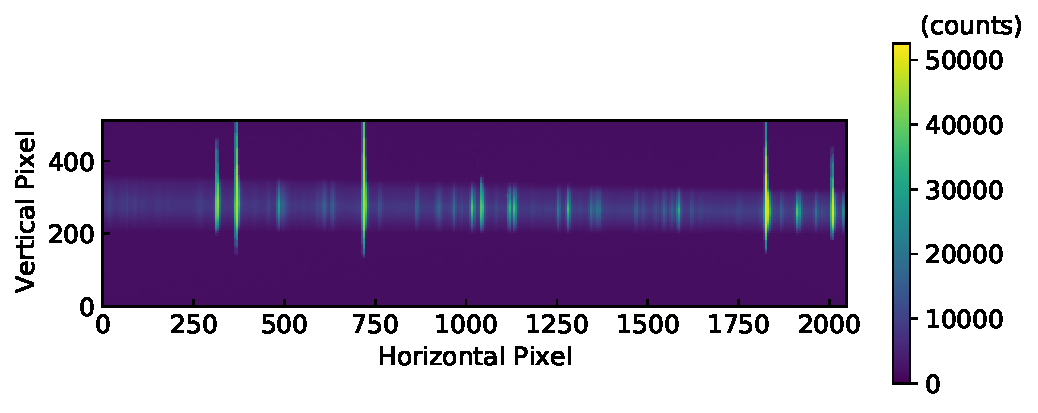
\includegraphics[width=15cm]{pictures/picture-example.pdf}
    \caption{CCDカメラで撮影した602.2-611.2 nmの波長範囲に対応する画像}
    \label{fig:picture-example}
\end{figure}

\begin{figure}
    \centering
    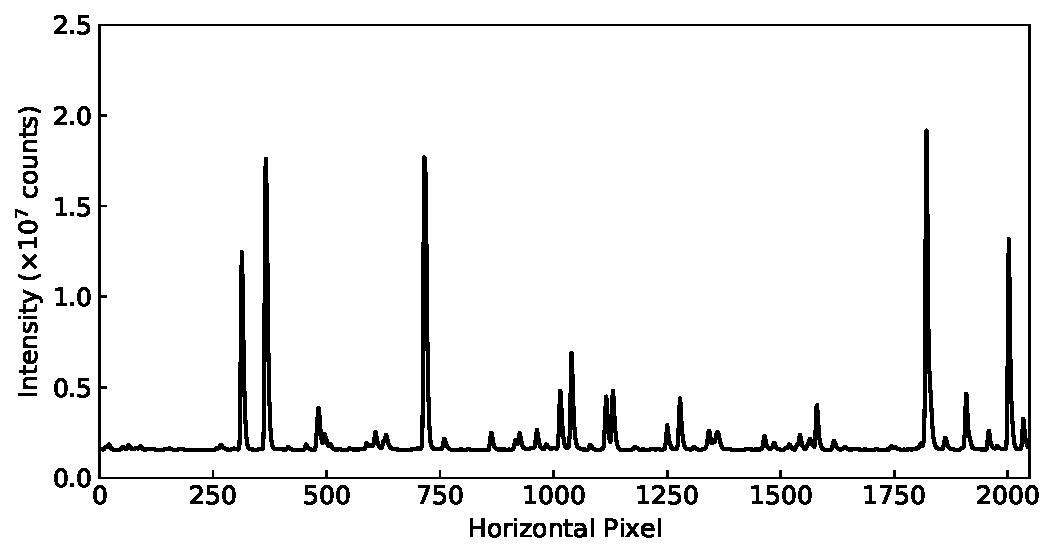
\includegraphics[width=15cm]{pictures/spectrum-example.pdf}
    \caption{図\ref{fig:picture-example}の画像を縦方向に0-506 ピクセルの範囲でビニングして得られたスペクトル}
    \label{fig:spectrum-example}
\end{figure}

\begin{figure}
    \centering
    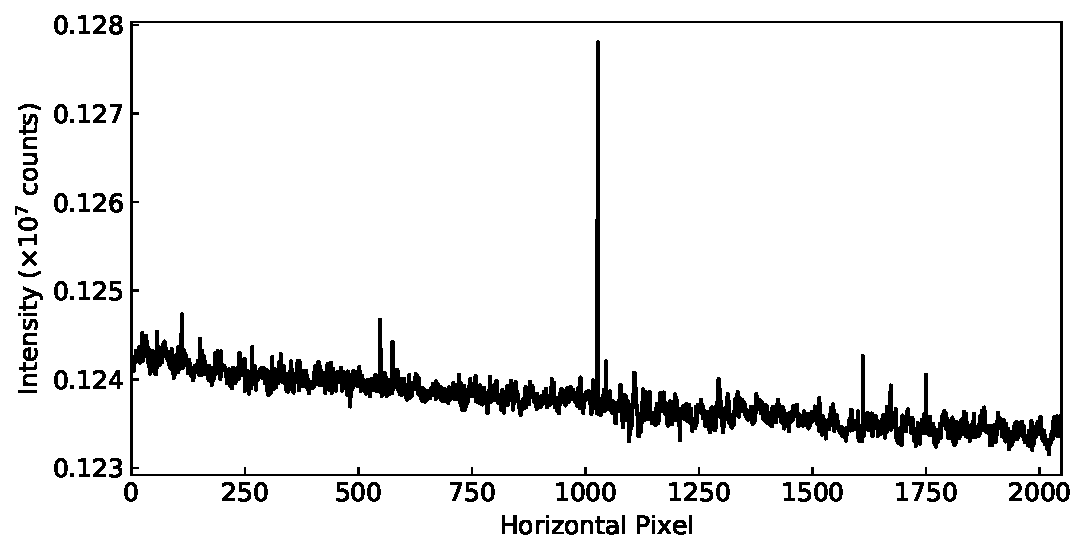
\includegraphics[width=15cm]{pictures/back-spectrum-example.pdf}
    \caption[プラズマを消した状態で得た画像を縦方向に0-506 ピクセルの範囲でビニングして得られたスペクトル]{プラズマを消した状態で得た画像を縦方向に0-506 ピクセルの範囲でビニングして得られたスペクトル.横方向に1027番目のピクセルは不良ピクセルである.}
    \label{fig:back-spectrum-example}
\end{figure}

\begin{figure}
    \centering
    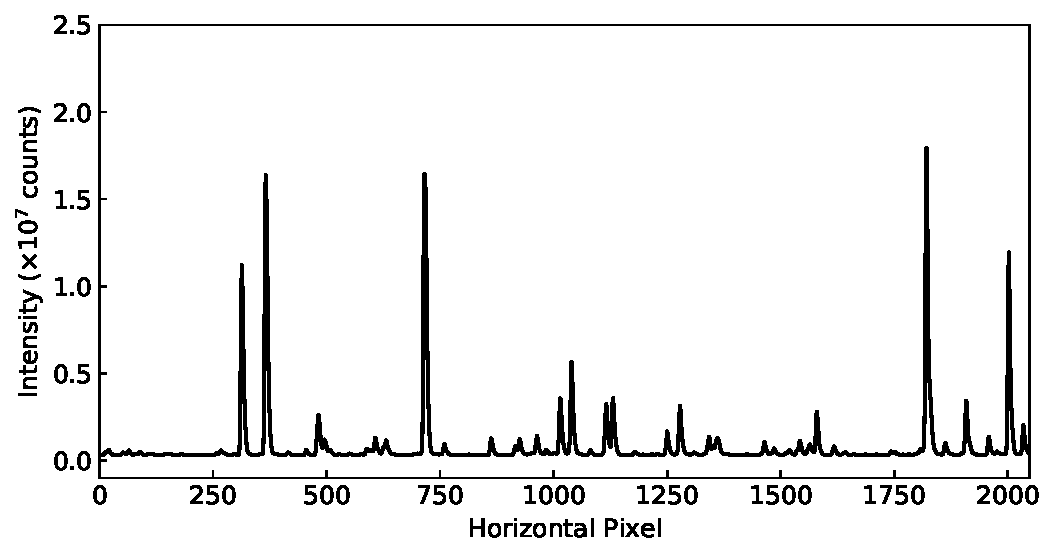
\includegraphics[width=15cm]{pictures/true-spectrum-example.pdf}
    \caption{図\ref{fig:spectrum-example}からバックグラウンドを除いたスペクトル}
    \label{fig:true-spectrum-example}
\end{figure}

\begin{figure}
    \centering
    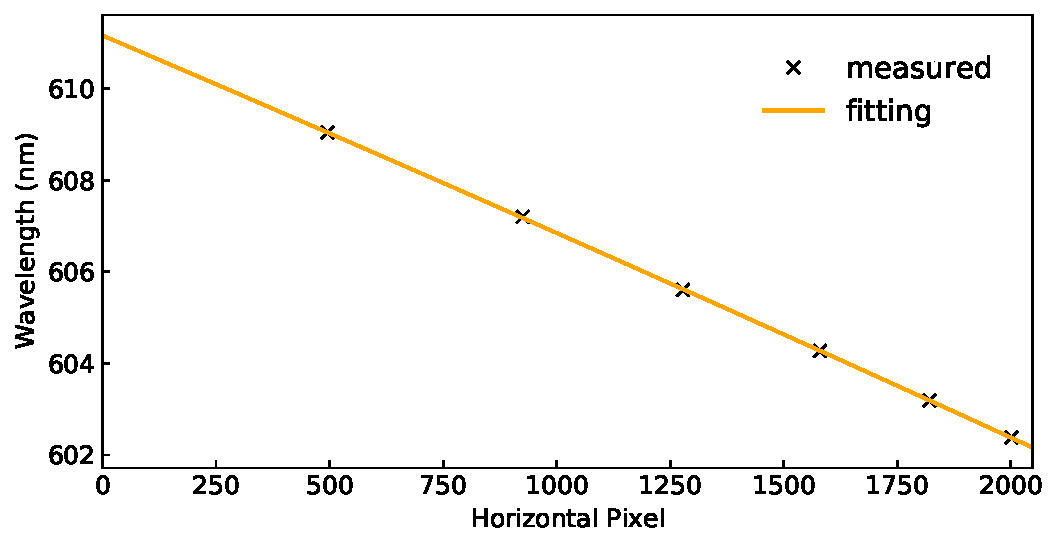
\includegraphics[width=15cm]{pictures/pixel-to-wavelength.pdf}
    \caption{図\ref{fig:true-spectrum-example}から求めたピクセル値と波長の対応関係}
    \label{fig:pixel-to-wavelength}
\end{figure}

\begin{figure}
    \centering
    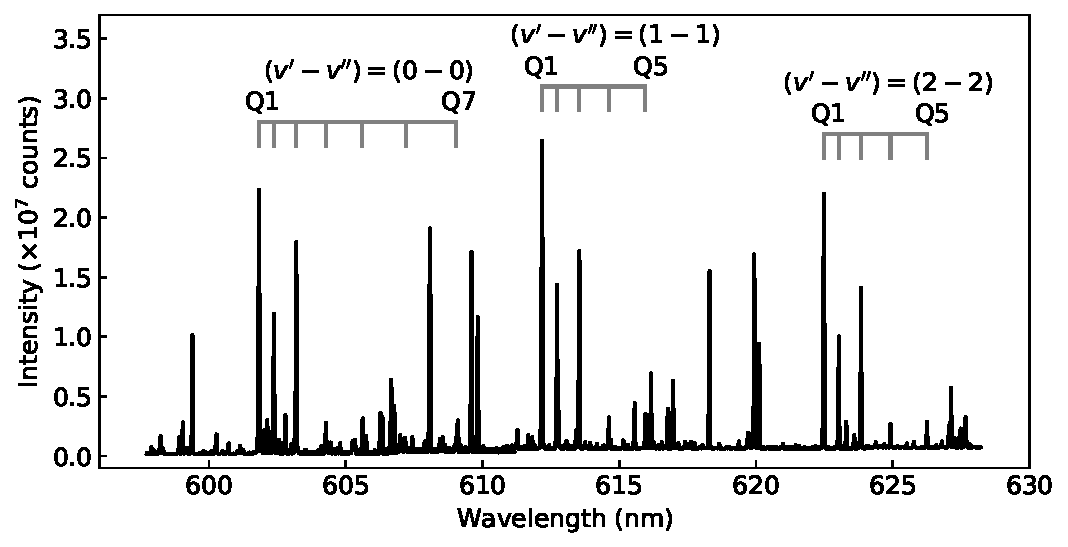
\includegraphics[width=15cm]{pictures/all-spectrum.pdf}
    \caption{Fulcher-α帯Q枝発光スペクトル}
    \label{fig:all-spectrum}
\end{figure}

\begin{figure}
    \centering
    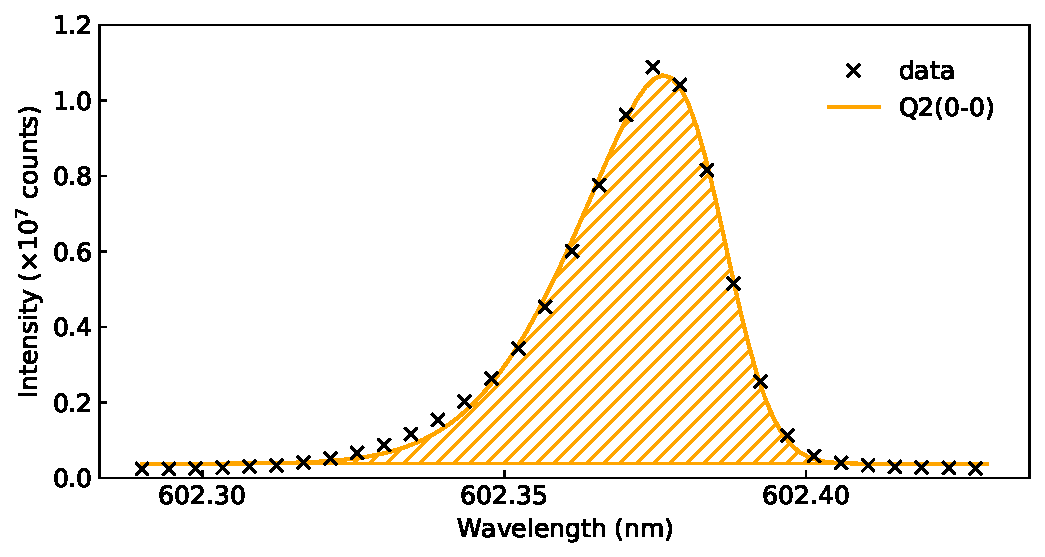
\includegraphics[width=15cm]{pictures/skewed-gaussian-fitting-00_Q2.pdf}
    \caption{Q2(0-0)発光線の歪正規分布関数によるフィッティング結果}
    \label{fig:voigt-fitting-1}
\end{figure}

\begin{figure}
    \centering
    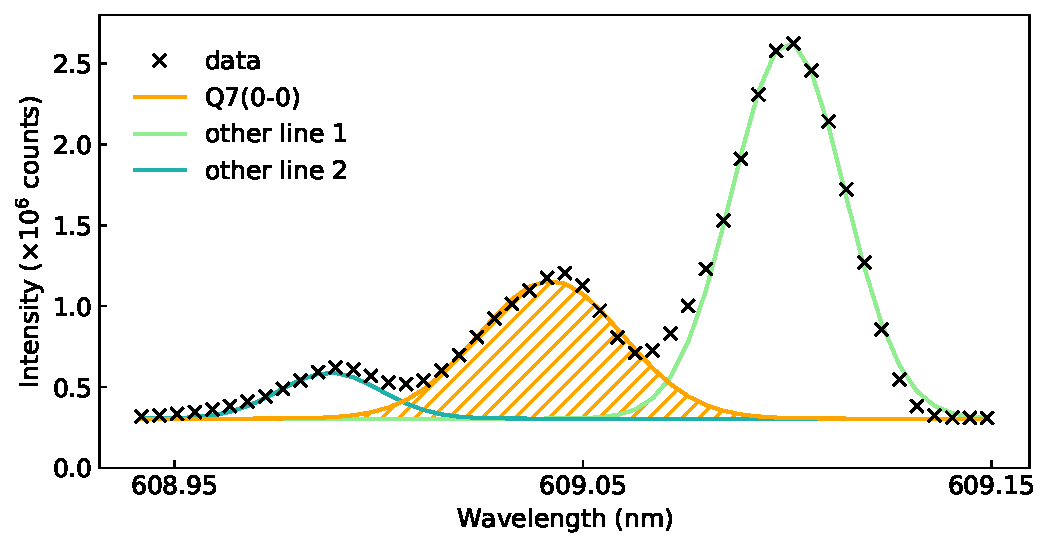
\includegraphics[width=15cm]{pictures/skewed-gaussian-fitting-00_Q7.pdf}
    \caption{Q7(0-0)発光線の歪正規分布関数フィッティングによる分離}
    \label{fig:voigt-fitting-2}
\end{figure}

\begin{figure}
    \centering
    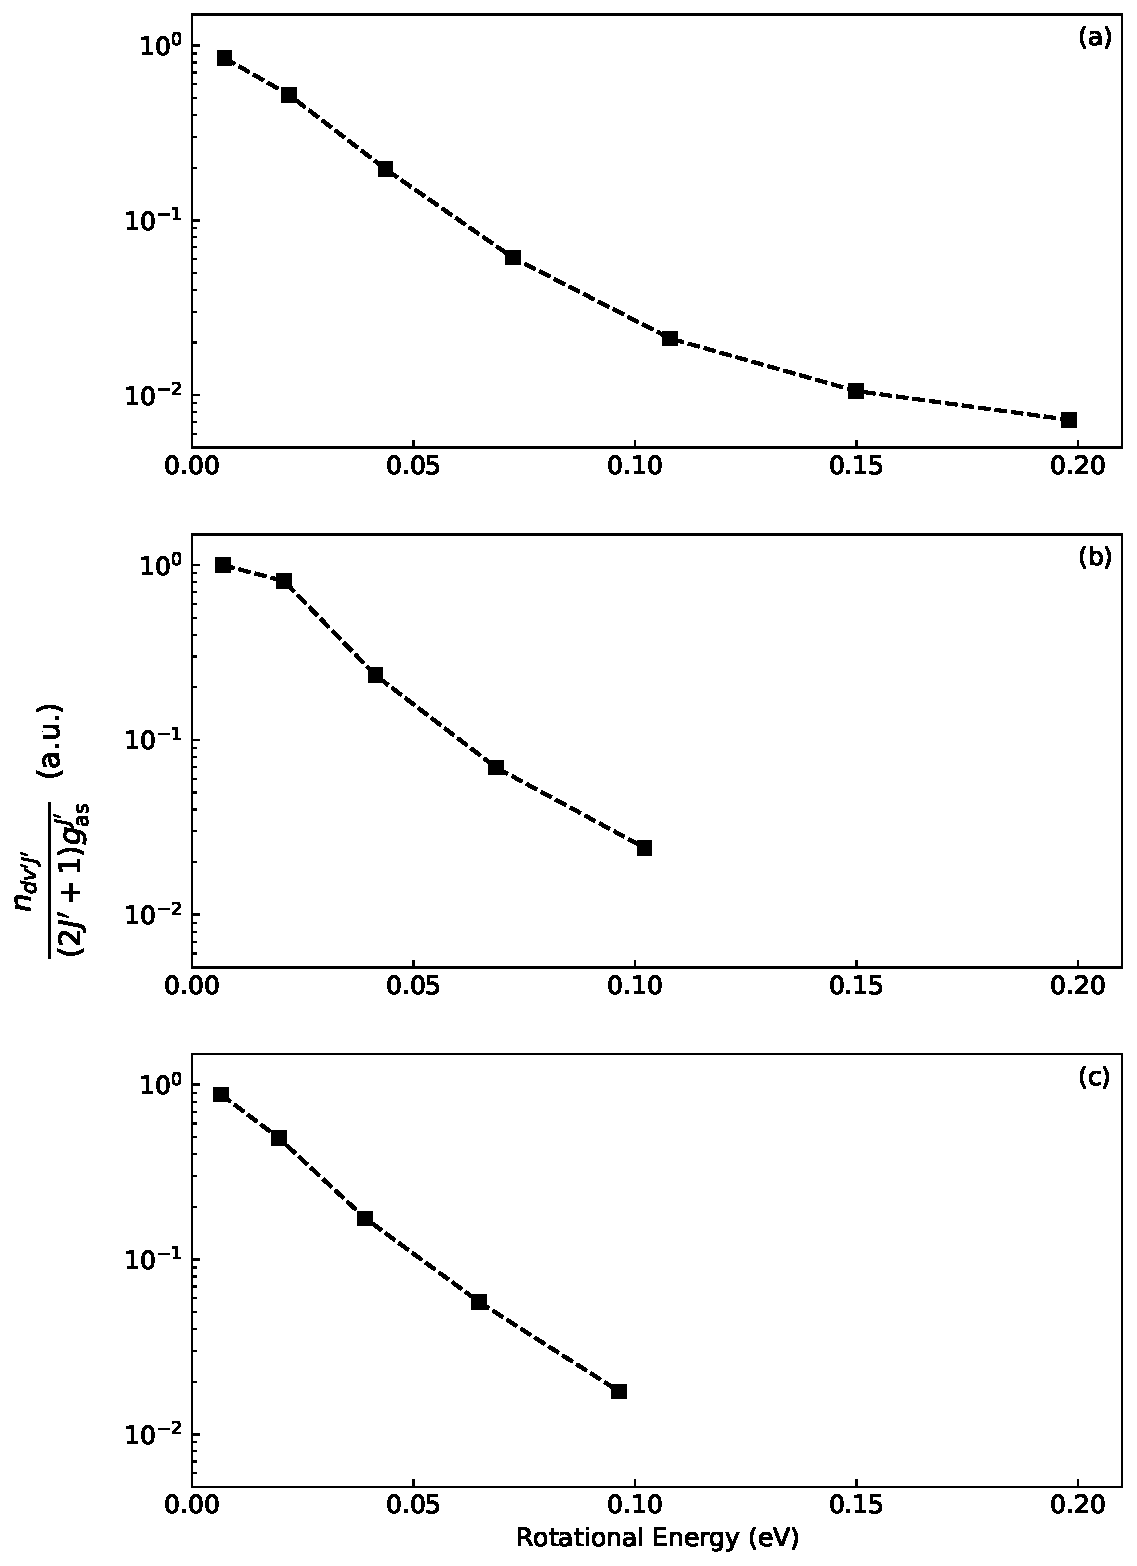
\includegraphics[width=15cm]{pictures/upper-boltzmann-plot.pdf}
    \caption{発光上準位における振動・回転状態占有率の回転エネルギー依存性}
    \label{fig:upper-boltzmann-plot}
\end{figure}

\begin{figure}
    \centering
    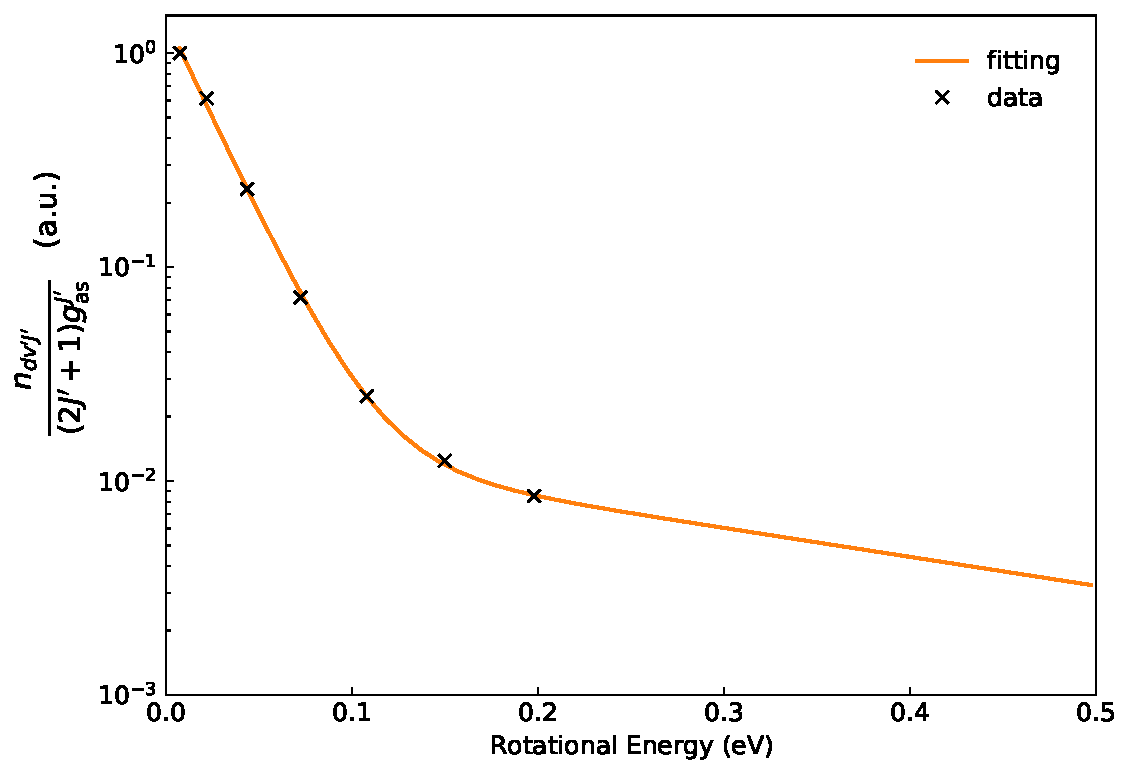
\includegraphics[width=15cm]{pictures/upper-two-fitting.pdf}
    \caption{発光上準位の振動準位$v'=0$における振動・回転状態占有率の2温度ボルツマン分布によるフィッティング結果}
    \label{fig:two-boltzmann-fitting}
\end{figure}

\begin{figure}
    \centering
    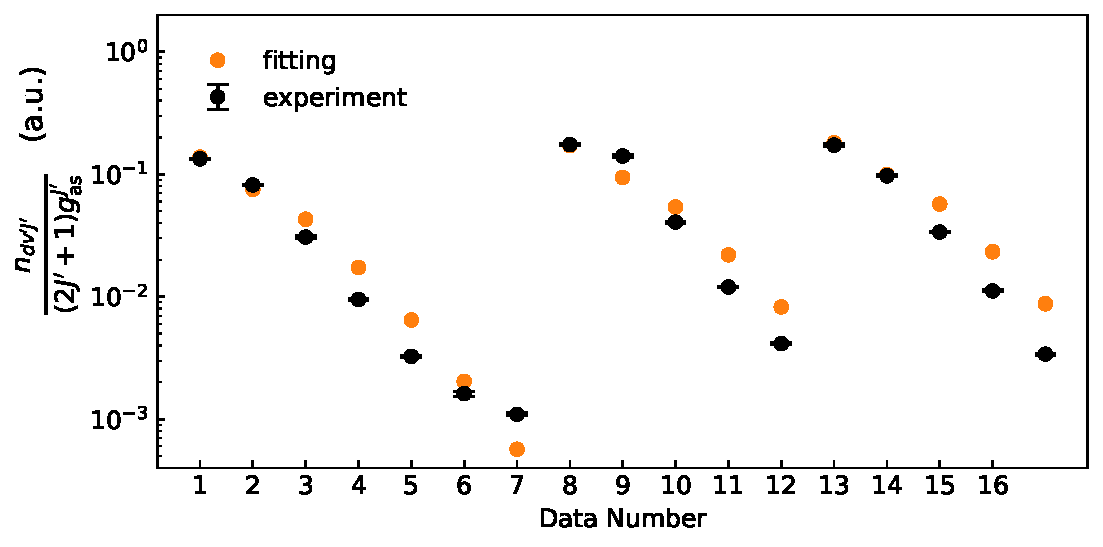
\includegraphics[width=15cm]{pictures/fitting-result.pdf}
    \caption[発光上準位における振動・回転状態占有率のコロナモデルによるフィッティング結果]{発光上準位における振動・回転状態占有率のコロナモデルによるフィッティング結果.横軸は解析に使用したデータの順番を表し,1〜15まで順に($v',J'$)=(0,1)〜(0,5),(1,1)〜(1,5),(2,1)〜(2,5)となっている.}
    \label{fig:fitting-result}
\end{figure}

\begin{figure}
    \centering
    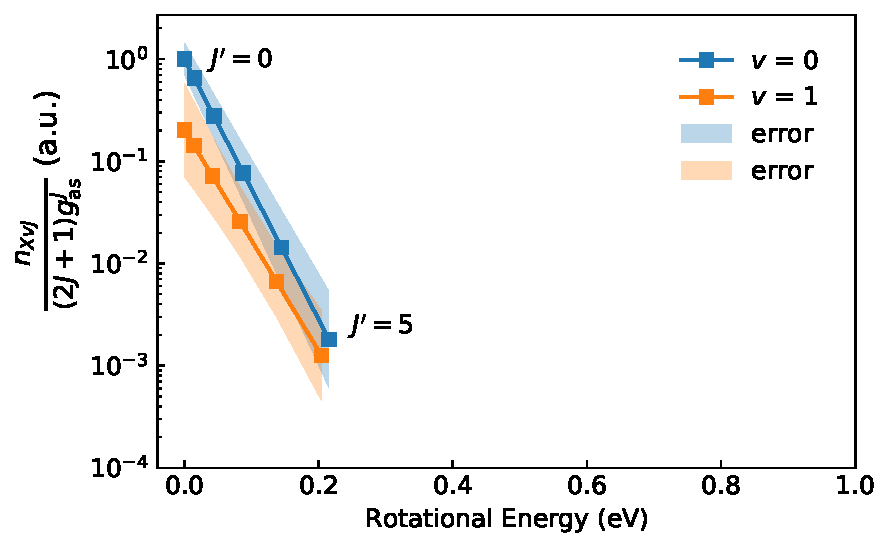
\includegraphics[width=15cm]{pictures/ground-state-gosa.pdf}
    \caption{基底準位における振動・回転状態占有率の回転エネルギー依存性}
    \label{fig:ground-state-n}
\end{figure}

\begin{figure}
    \centering
    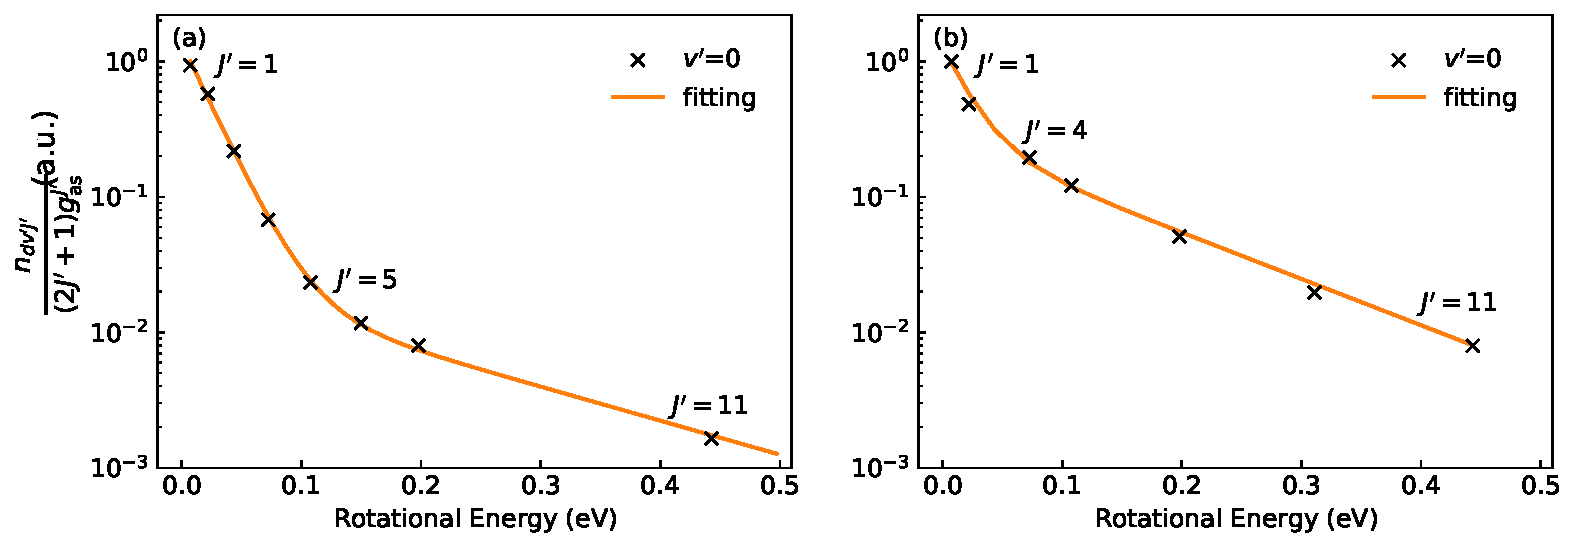
\includegraphics[width=15cm]{pictures/two-boltzmann-compare.pdf}
    \caption{本研究対象のプラズマとLHD\cite{ishihara}での発光上準位の振動準位$v'=0$における振動・回転状態占有率の回転エネルギー依存性}
    \label{fig:two-boltzmann-compare}
\end{figure}

\begin{figure}
    \centering
    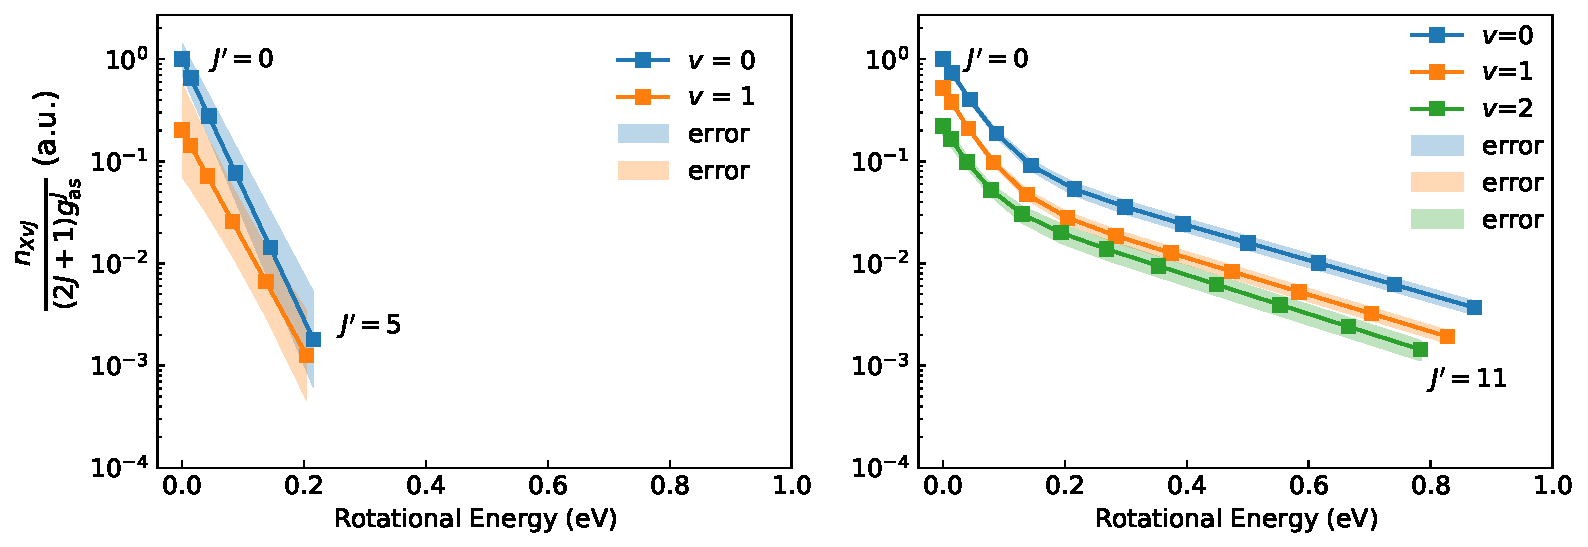
\includegraphics[width=15cm]{pictures/ground-compare.pdf}
    \caption{本研究対象のプラズマとLHD\cite{ishihara}での基底準位における振動・回転状態占有率の回転エネルギー依存性}
    \label{fig:ground-compare}
\end{figure}
